\documentclass[11pt]{article}
\usepackage{amsmath,textcomp,amssymb,geometry,graphicx,verbatim,enumerate}
\usepackage{fancyhdr}
\pagestyle{fancy}
\def\Names{Davis Foote, Ajeya Cotra, Leah Dickstein, Ena Hariyoshi}
\def\Session{Fall 2014}

\title{EE126--Fall 2014 --- Mini-Project Extras}
\author{\Names}
\lhead{EE126--\Session\ Extras--\Names}

\begin{document}
\maketitle
In this document you will see the fruits of an attempt to analytically solve for the probability that all the moths will turn grey given a specified starting state. Using the notation specified in our write-up, we drew the smallest possible example that would still be interesting:
\begin{center}
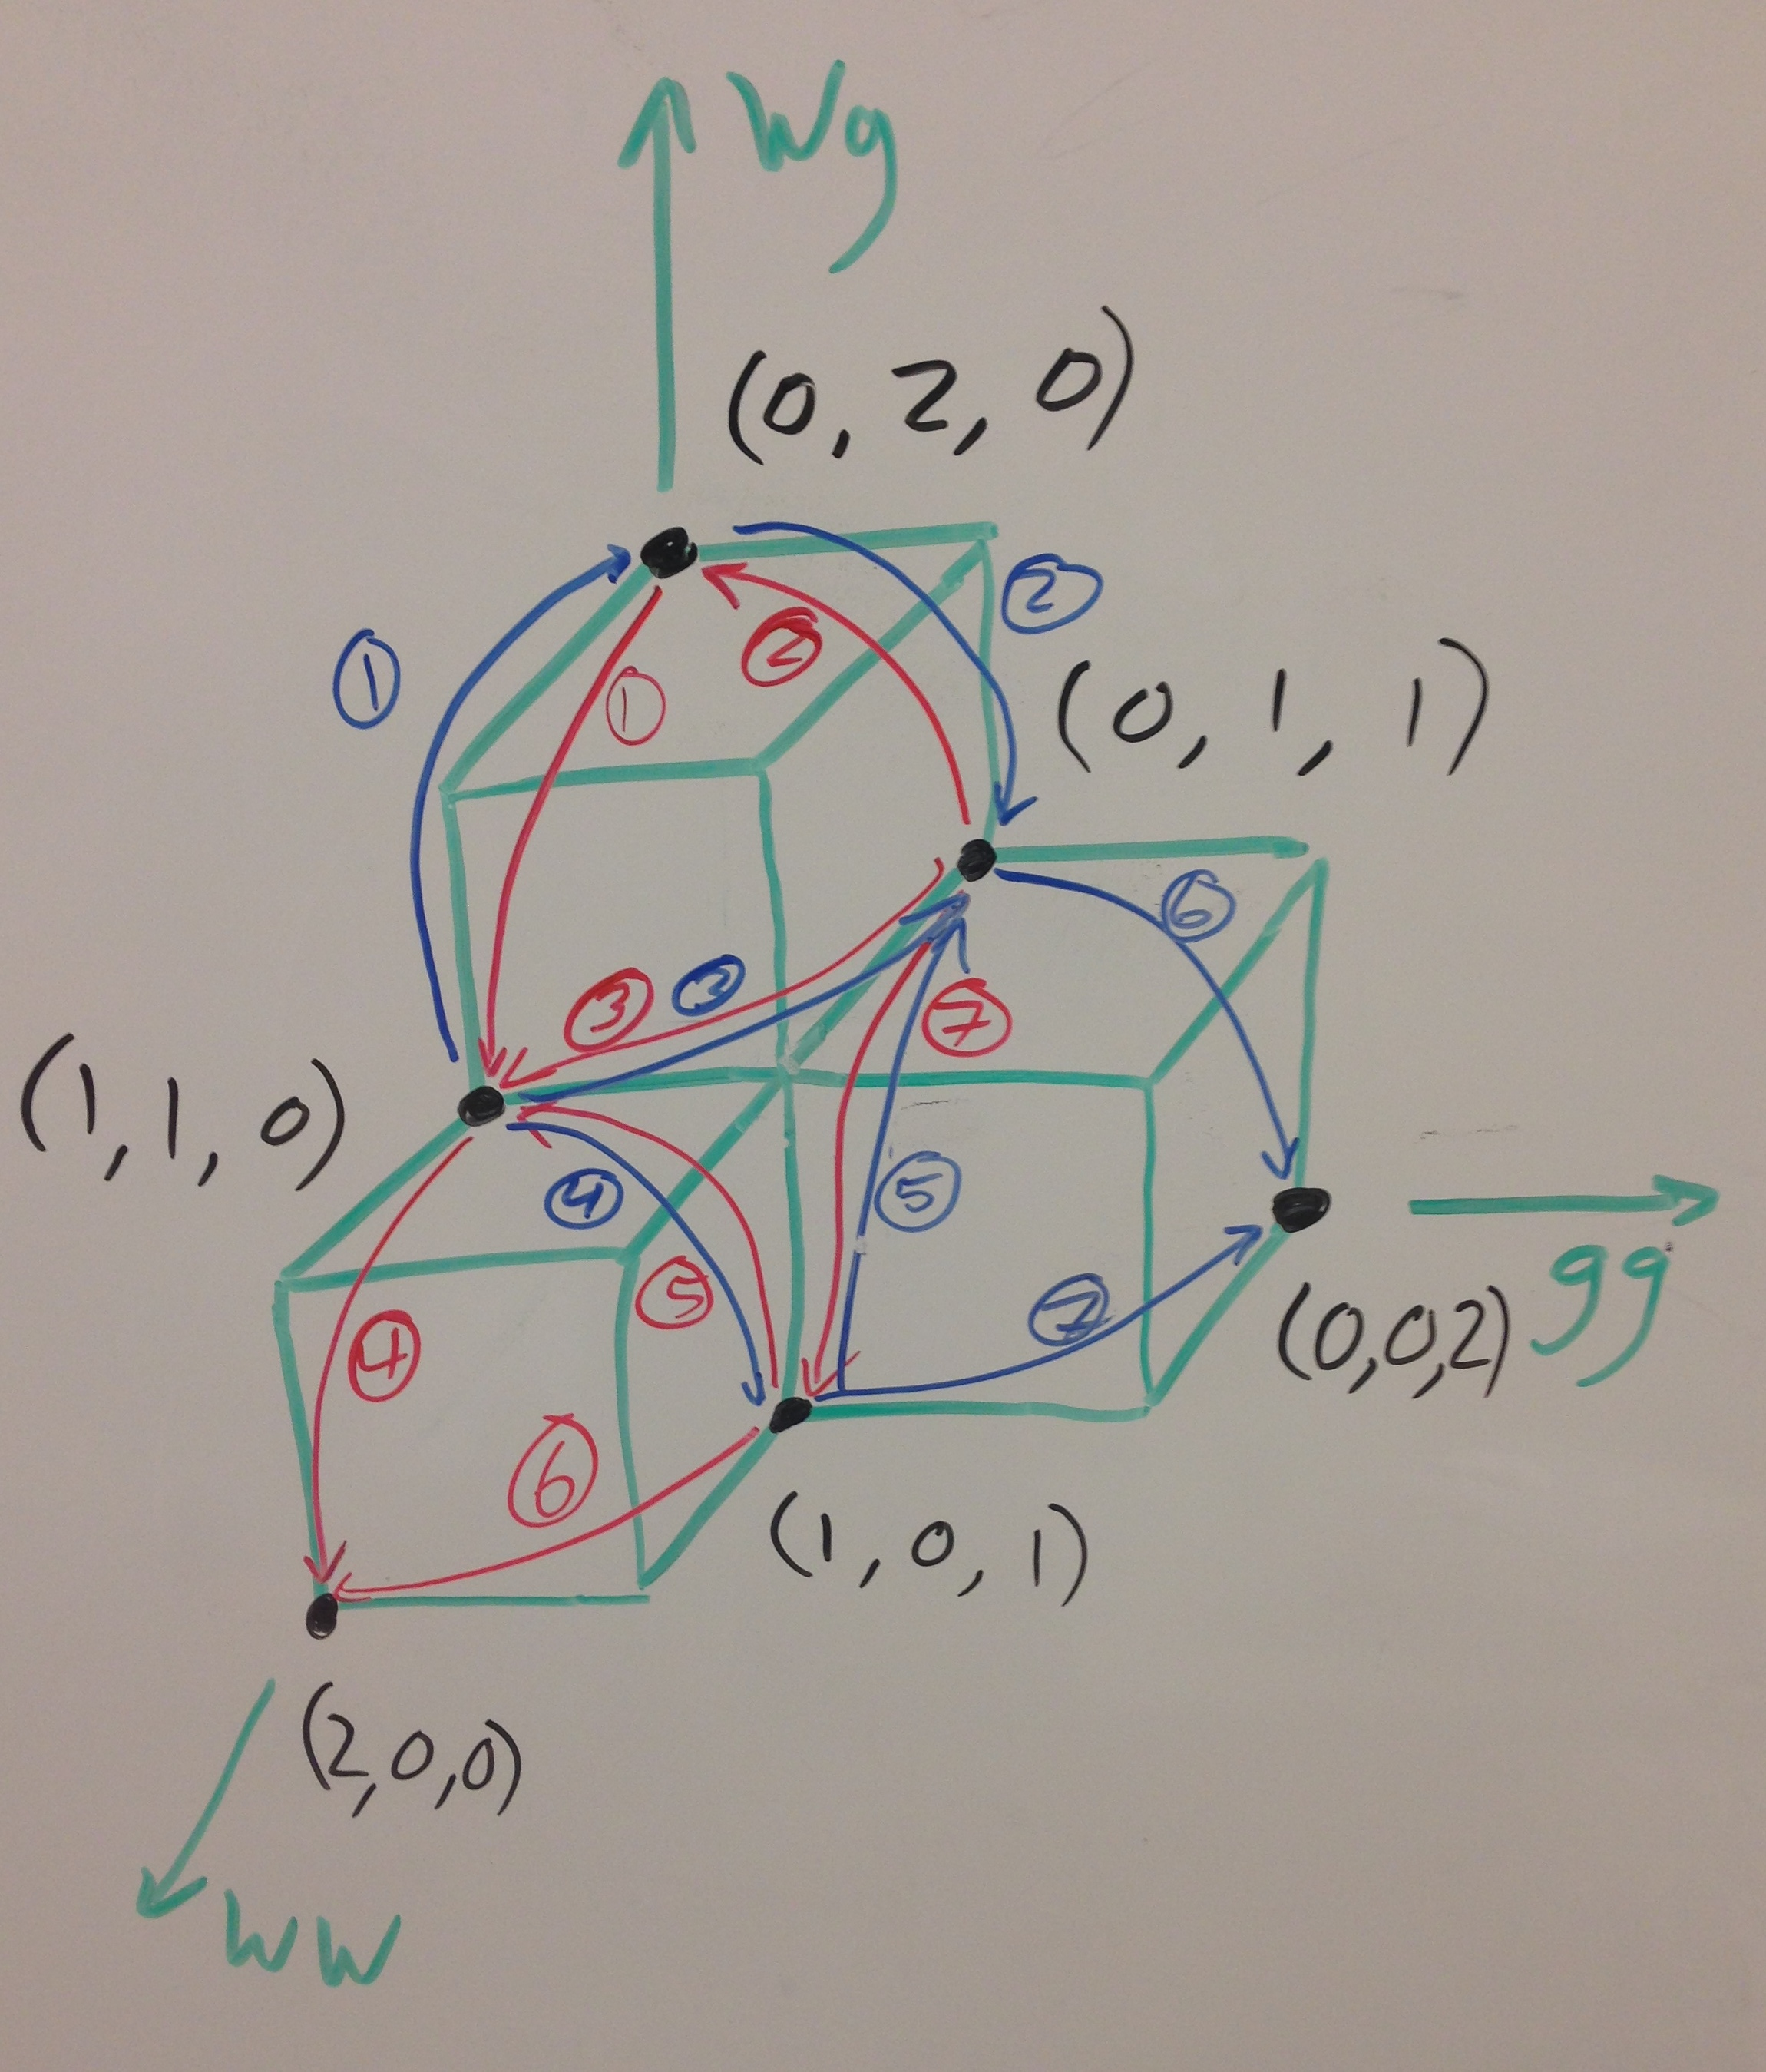
\includegraphics[scale=0.1]{markov-chain}
\end{center} 

We then defined, for each state in the M.c., a probability that the state $(0,0,2)$ would eventually be reached. The arrows are drawn in red and blue to differentiate the ones going left and right. The transition probabilities corresponding to the red probabilities are referred to with $b_is$, and those corresponding to the blue transitions are referred to with $a_is$. The resulting system of equations is as follows: \newpage

\begin{center}
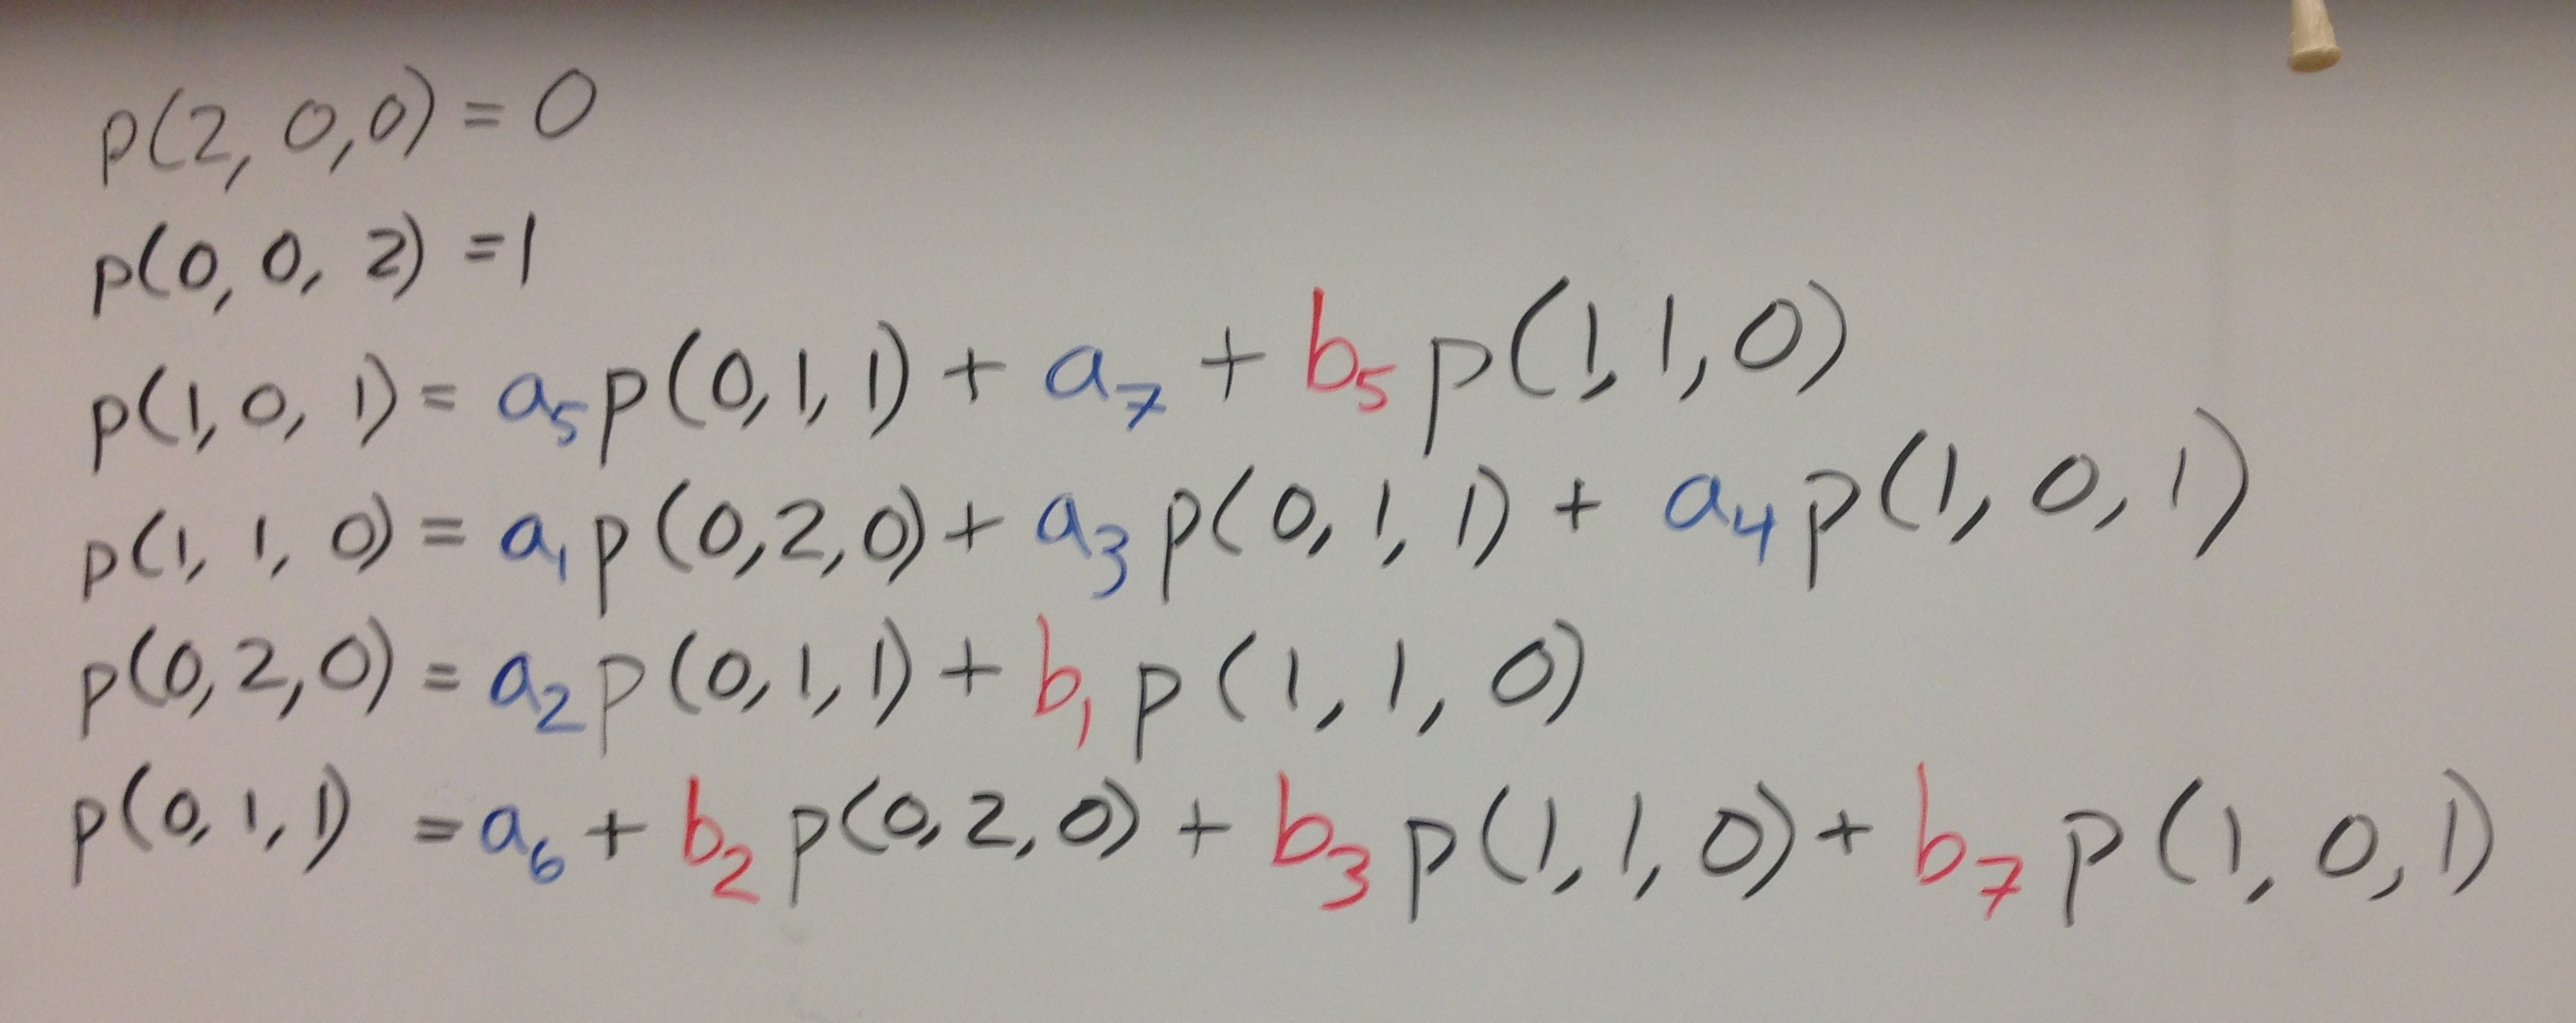
\includegraphics[scale=0.1]{equations}
\end{center}

We then set up the augmented matrix:

\begin{center}
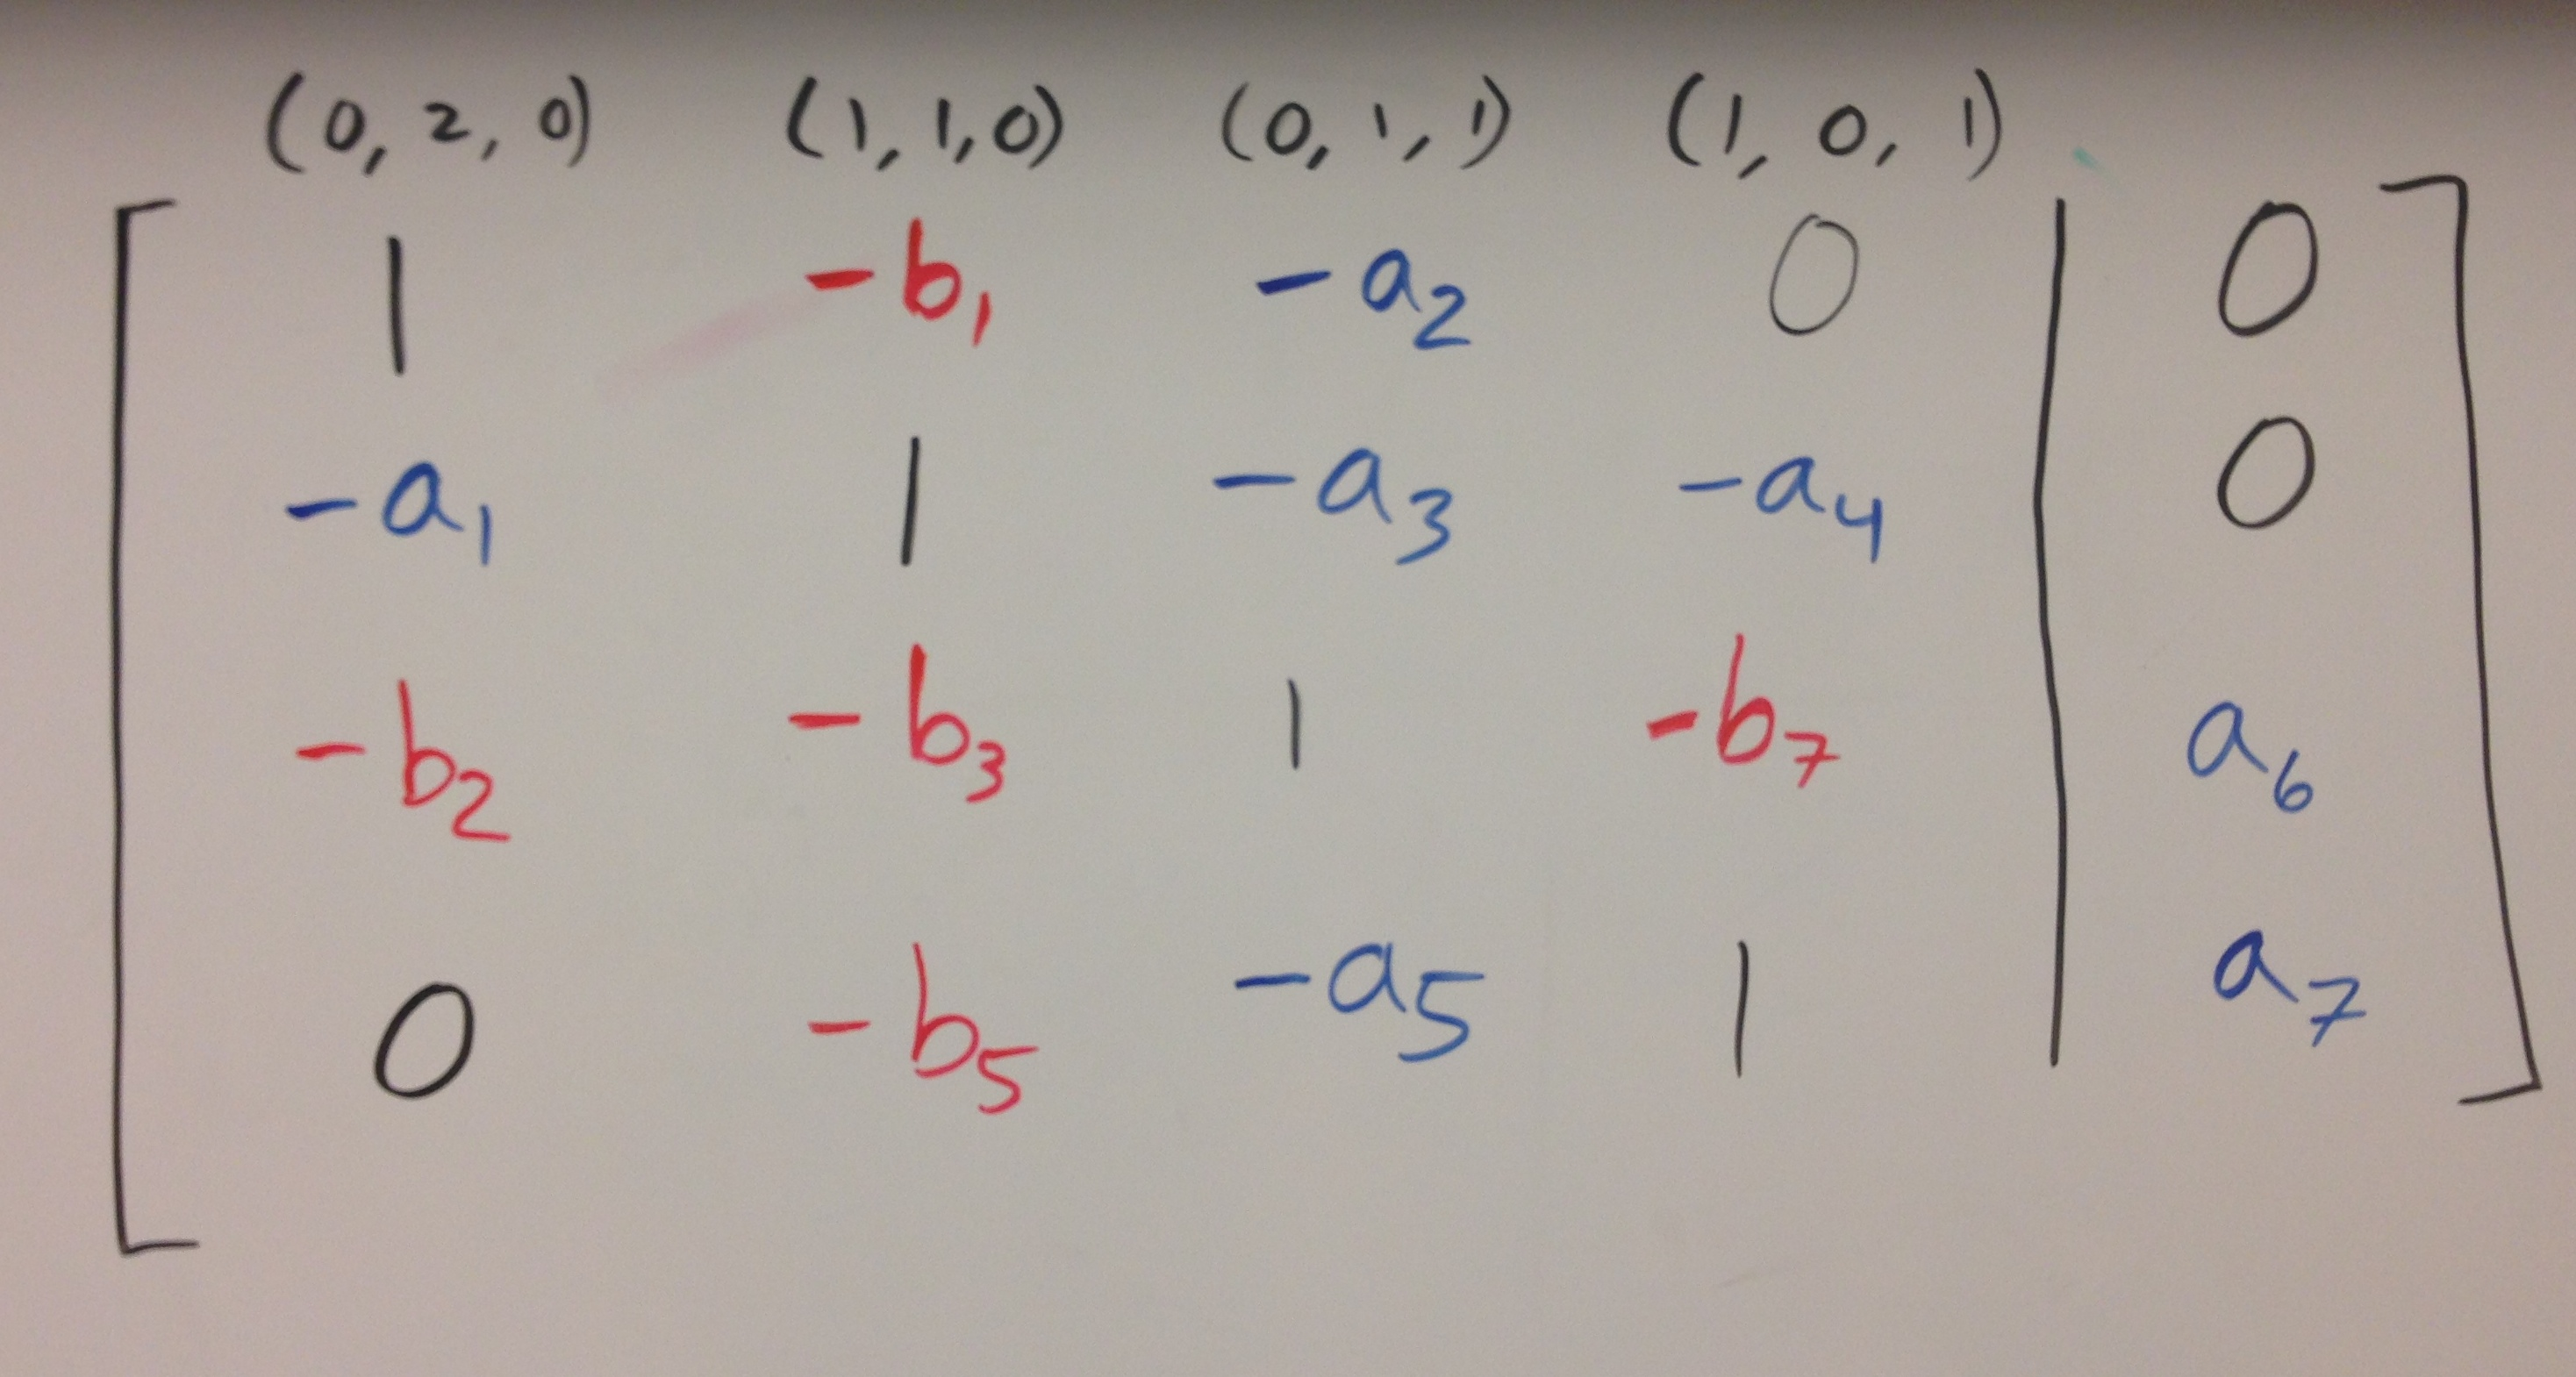
\includegraphics[scale=0.1]{matrix}
\end{center}

Once we have a solution in terms of the transition probabilities $a_i$ and $b_i$, we can solve for the transition probabilities using the method described in out project write-up to get a final analytical solution for the probabilities of all the moths turning grey from a given starting position. We enter the matrix into Wolfram Alpha to be row-reduced:
\begin{center}
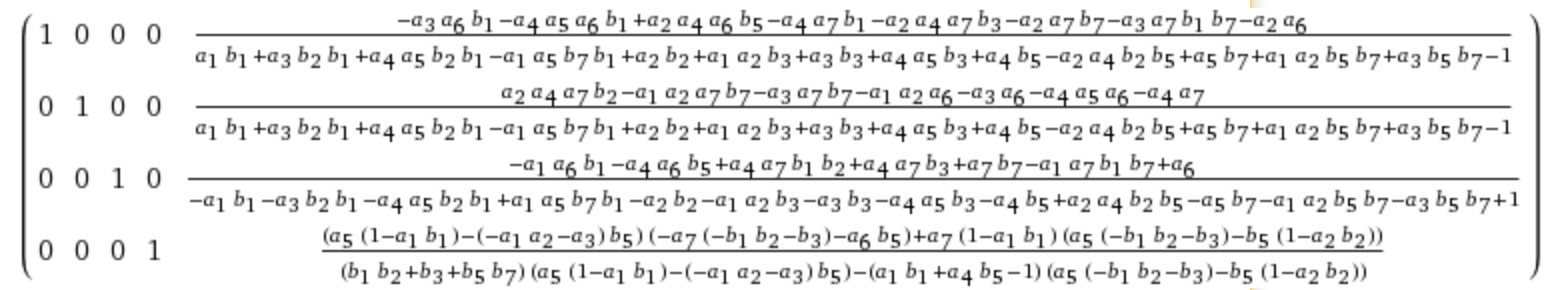
\includegraphics[scale=0.6]{wolfram}
\end{center}
And thus concludes the story of why we did not solve for the probability analytically.
\begin{center}

\includegraphics[scale=0.5]{the-end}
\end{center}
\end{document}